\chapter{Introduction}
\label{chapter:introduction}

The decisive role of optimized and robust software in safety and mission-critical distributed real-time embedded (DRE) systems is becoming increasingly recognized. Embedded software is pertinent in a variety of heterogeneous domains e.g. avionics \cite{burke2010distributed}, automotive systems \cite{navet2008automotive}, locomotives \cite{zimmermann2003train}, and industrial control systems \cite{zoitl2008real}. The volume and complexity of such software grows everyday depending on an assortment of factors, including challenging system requirements e.g. resilience to hardware and software faults, remote deployment and repair. Deployment, the procedure for launching or reconfiguring software processes on embedded hardware, becomes extremely difficult if obtaining access to such devices is limited. Large scale deployment of embedded software, for this reason, has become considerably more arduous -- periodic peer reviews, numerous verification and certification methods are applied to maintain industry standards for safety, precision and reliability of embedded real-time software. Even still, software errors manifest in deployed systems; errors that can be extremely difficult to reproduce in a laboratory test environment. 

There exists a long list of real-world scenarios where errors in embedded software implementations has cost millions of dollars and human life. Between 1999 and 2010, at least 2,200 Toyota vehicles sold in the United States experienced unintended cases of rapid acceleration, causing nearly 900 accidents and over 100 deaths \cite{Cusumano:2011:RTD:1866739.1866750}. In 2010, Toyota recalled some 10 million vehicles, an extraordinary number given that the company sold only about seven million vehicles during that period. Toyota engineers described the problem as a disconnect in the vehicle's complex anti-lock brake system (ABS) that causes less than a one-second lag in its operation. With this delay, a vehicle going 60 mph will have traveled nearly another 90 feet before the brakes begin to take hold. Brakes in Toyota hybrids such as the Prius operate differently from brakes in most cars. In addition to the standard brakes, which use friction from pads pressed against rotors, the embedded software driving the electric motors help slow the vehicle. This process also generates electricity to recharge the batteries. This is a prime example of how timing errors in consumer-focused embedded software, spanning millions of lines of code, can have disastrous effects to everyday life. The Prius is Toyota's third best-selling model in the United States. The automaker recalled 2.3 million vehicles on January, 2011 because of problems with sticking gas pedals and later halted the sale of the eight models involved in the recall. Toyota's U.S. sales plunged 16 percent in January as a result, even as sales of other automakers rose.

To mitigate such software complexity, model-driven component-based software engineering (CBSE) and development \cite{beydeda2005model, heineman2001component, clemens1998component, simulink1993mathworks, autosar} has become an accepted practice. CBSE tackles escalated demands with respect to requirements engineering, high-level design, error detection, tool integration, verification and maintenance. The widespread use of component technologies in the market has made CBSE a focused field of research in the academic sectors. Applications are built by assembling together small, tested component building blocks that implement a set of services. These building blocks are typically built from UML \cite{UML} class diagrams, or imported from other projects/vendors and \emph{connected} together via exposed interfaces, providing a "black box" approach to software construction. This approach also treats software verification in a more modular fashion; the various software components can be verified individually and then composed together to derive a functional system. 

Remote embedded devices e.g. fractionated spacecraft \footnote{A fractionated spacecraft is a satellite architecture where the functional capabilities of a conventional monolithic spacecraft are distributed across multiple modules which interact through wireless network links.} following mission timetables and hosting distributed software applications expose several concerns including strict timing requirements, complexity in deployment, repair and integration; and resilience to faults, including mechanical failures like surface fractures, electrical failures such as single-event upsets, and manufacturing defects, and lastly software failures such as design defects and run-time faults. High-security and time-critical software applications hosted on such platforms run concurrently with all of the system-level mission management and fault recovery tasks that are periodically undertaken on the distributed nodes. Once deployed, it is often difficult to obtain a reliable period of low-level access to such remote systems for runtime debugging and evaluation. These types of DRE systems, therefore demand comprehensive design-time modeling and analysis methods to detect possible anomalies in system behavior, like the unacceptable response times in the advanced braking systems in vehicles. 

With the DARPA System F6 Project, our team has designed and prototyped a full information architecture called \emph{\textbf{D}istributed \textbf{RE}al-time \textbf{M}anaged \textbf{S}ystems} (DREMS) \cite{ISIS_F6_Aerospace:12,DREMS13Software} that addresses requirements for rapid component-based application development and deployment for fractionated spacecraft. The stack of developed software includes a  design-time model-driven development tool suite \cite{ISIS_F6_SFFMT:13}, and a component model \cite{ISIS_F6_ISORC:13} with precise execution semantics enabling robust and analyzable software designs. The minutiae of the DREMS architecture are described in Chapter \ref{chapter:DREMS}. The formal modeling and analysis methodology presented in this dissertation focuses on applications that rely on this foundational architecture. 

The principle behind design-time analysis here is to map the structural and behavioral specifications of the system under analysis into a formal domain for which analysis tools exist. The key is to use an appropriate model-based abstraction such that the mapping from one domain to another remains valid under successive refinements in system development such as code generation. The analysis must ensure that as long as the assumptions made about the system hold, the behavior of the system lies within the safe regions of operation. The results of this analysis will enable system refinement and re-design if required, before actual code development. 

\begin{figure}
	\centering
	\begin{subfigure}{.5\textwidth}
		\centering
		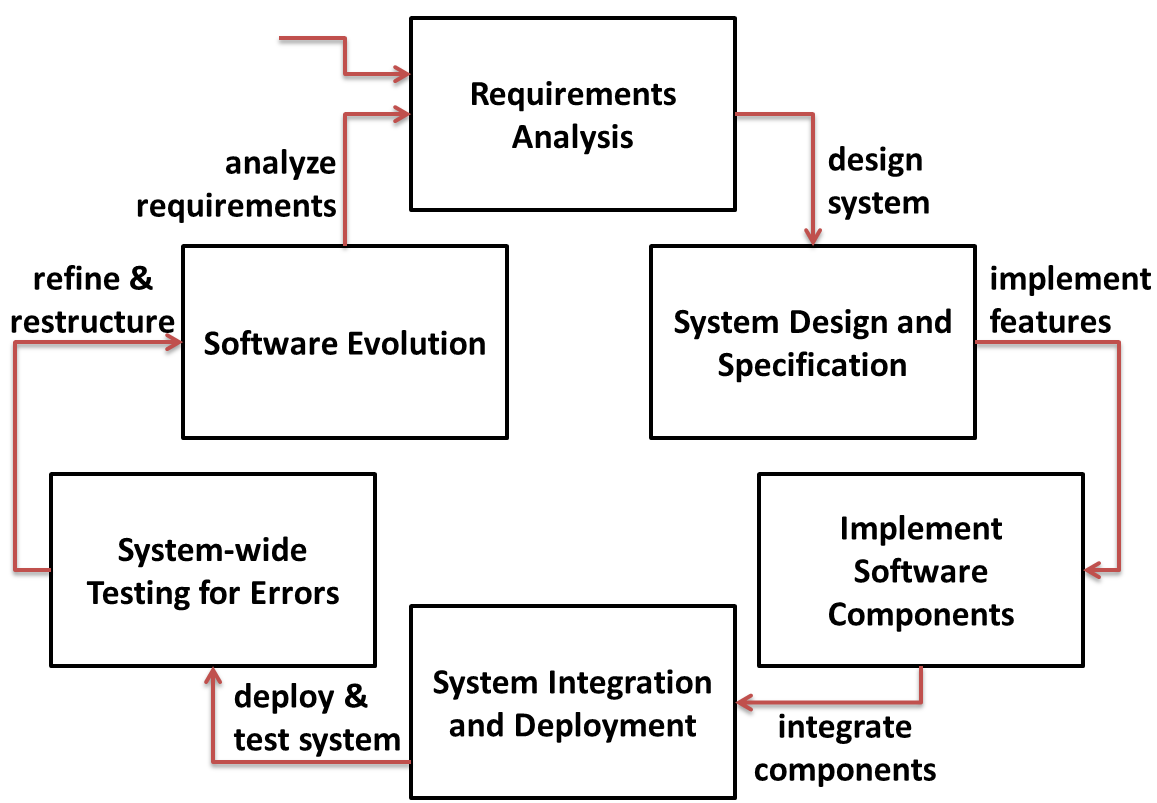
\includegraphics[width=0.9\linewidth]{sdlc}
		\caption{Industrial SDLC}
		\label{fig:sdlc}
	\end{subfigure}%
	\begin{subfigure}{.5\textwidth}
		\centering
		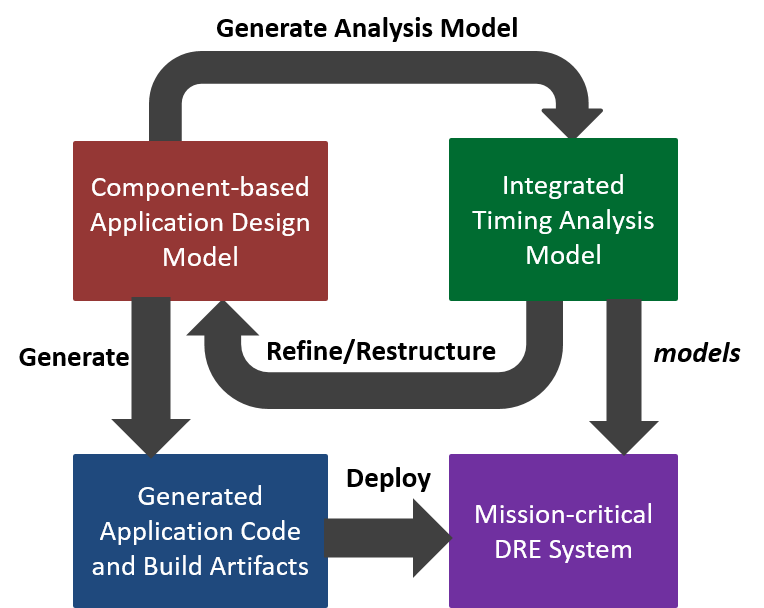
\includegraphics[width=\linewidth]{big_picture_2}
		\caption{DREMS Analysis-driven Workflow}
		\label{fig:big_picture}
	\end{subfigure}
	\caption{Embedded Software Development Lifecycle Comparison}
	\label{fig:test}
\end{figure}

Figure \ref{fig:sdlc} shows a \emph{spiral model} \cite{boehm1988spiral} of a typical industrial software/system development life cycle (SDLC). The five stages in this cycle include requirements analysis, software design, implementation, integration testing, and design evolution. Although the intricacies of each stage is hidden, the large majority of industrial software development follows this lifecycle. Embedded software development, especially for safety critical systems, does not lend itself well to this life cycle, mainly because the deliverable in such projects is usually not just a software package or a hardware platform but an amalgamation of both. Software development in fields like robotics, is tightly coupled with the hardware; assessment of software performance is sometimes dependent on and blocked by the hardware availability. Such blocking delays lead to inefficiencies in software evaluation and longer development times. It is also possible that design oversights could lead to poor timing performance e.g. long response times to critical events, that could damage the hardware in the process. Thus, the analysis presented in this work, supports and argues for a verification-driven workflow, as shown in Figure \ref{fig:big_picture}. The software evaluation is performed at design-time and as often as possible until the assembly is refined and optimized. Application developers use domain-specific modeling languages to structure large-scale component assemblies and modular code generation features to speed up software development efforts. Moreover, domain-specific properties such as interaction patterns, component execution code, and associated temporal properties such as worst-case execution times, deadlines etc. can be easily injected into such models. Using such application parameters in the \textit{design} model, a Colored Petri net-based (CPN) \cite{CPN} \textit{formal analysis model} is generated. The system behavior is both simulated and analyzed using a CPN execution engine, CPN Tools \cite{CPNTools}, and useful properties of the system are verified. By generating a bounded \emph{state space} of the system, the execution traces exhibited by the system are searched for property violations. Such system properties include the lack of deadlocks, deadline violations and worst-case trigger-to-response times. The goal of this analysis is to ensure that a component-based system: an assembly of tested component building blocks, meets the temporal specifications and requirements of the system.  

The results of this analysis will help improve the structure of the application, enabling safe deployment of dependable components that are known to operate within system specifications. Using CBSE also enables this restructuring process as the components are not tightly coupled software entities. So, when designing the integrated system, the analysis can be performed by assigning \emph{time budgets} to the discrete tasks in the execution. This enables timing analysis before implementation and also uses the time budgets as requirements for efficient code implementation. These budgets are often derived from some high-level requirements and appropriately distributed between the different components in the system. The analyzed system may not necessarily be complete, but instead be in a process of evolution. As the design progresses, the system requirements become concrete and the design is re-verified at each stage to ensure the consistency of all timing guarantees. 

The remainder of this dissertation is organized as follows. Chapter \ref{chapter:fundamentals} describes some fundamental concepts about distributed real-time systems, component-based software and some challenges in timing analysis. Chapter \ref{chapter:related-research} briefly describes general software testing and analysis methodologies, and summarizing related research in timing analysis and verification for distributed real-time embedded applications. Chapter \ref{chapter:DREMS} introduces the DREMS infrastructure and the Component Model used to experiment with and validate the timing analysis results. Chapter \ref{chapter:modeling} discusses the Colored Petri net-based timing analysis model devised for component-based DRE systems. Chapter \ref{chapter:analysis} describes the scope and efficiency of the analysis methods implemented with this CPN model. Chapter \ref{chapter:evaluation} evaluates this model with published results on analysis design, scalability and experimental validation. Chapter \ref{chapter:conclusion} concludes the dissertation, providing a summary of the detailed work. Finally, Chapter \ref{chapter:publications} lists relevant publications.